\documentclass[11pt]{article}
\usepackage[margin=1in]{geometry}
\usepackage{amsmath,amssymb,booktabs,graphicx,hyperref,natbib}
\usepackage[T1]{fontenc}
\hypersetup{
  colorlinks=true,
  linkcolor=blue,
  citecolor=blue,
  urlcolor=blue,
  pdftitle={Likelihood-Ranked Synthetic Selection in Self-Consuming Diffusion},
  pdfauthor={Muhammad Alamzeb},
  pdfsubject={Model collapse; self-consuming diffusion; likelihood ranking},
  pdfkeywords={diffusion, model collapse, synthetic data, minority modes}
}

\title{Likelihood-Ranked Synthetic Selection in Self-Consuming Diffusion:\\
Minority Extinction Ordering on Imbalanced Mixtures}
\author{
Muhammad Alamzeb\\
\textit{Independent researcher}\\
\texttt{shayankhanmahar@gmail.com}
}
\date{}

\begin{document}
\maketitle

\begin{abstract}
Self-consuming training loops---retraining generative models on their own outputs---can induce \emph{model collapse}, including loss of rare modes.
We study unlabeled selection of synthetic samples by a denoising likelihood proxy in self-consuming DDPM training on imbalanced mixtures.
Under matched real-mix ratio and matched synthetic budget, the first-generation minority-mass \emph{ratio} $r=m^{(1)}/m^{(0)}$ obeys
\[\mathrm{bottom}\text{-}k \;\;>\;\; \mathrm{random}\text{-}k \;\;>\;\; \mathrm{top}\text{-}k\]
on a primary matrix of \textbf{eight} seed--imbalance cells (seeds $\{0,1,2\}$ at $\rho\in\{5,10\}$ plus seeds $\{3,4\}$ at $\rho{=}5$ only; means $0.57/0.36/0.17$).
Paired contrasts vs.\ random-$k$ show large effects (Cohen's $d_z{\approx}1.0$) with Wilcoxon $p{\approx}0.042$ (Holm-adjusted $p{\approx}0.085$ for the two tests); we treat the ordering as supported by effect size and directional consistency, with small-$n$ caveats.
Likelihood top-$k$ also concentrates majority mass relative to random-$k$.
A hypothesized ``false stability'' pattern---top-$k$ \emph{improving} sliced $W_2$ while minorities die---is \textbf{not observed}: at generation~1, $\Delta W_2(\mathrm{top}-\mathrm{rand})>0$ on $8/8$ cells (Wilcoxon $p{\approx}0.014$).
Directional transfer checks on $8$D GMM and Digits-PCA ($3$ seeds each) match the same order.
We release configs, seeds, logs, and analysis code with the manuscript package.
\end{abstract}

\section{Introduction}
As synthetic data proliferates, generative models are increasingly trained on mixtures of real and model-generated samples.
Iterated self-consumption can cause \emph{model collapse}: progressive loss of diversity and forgetting of rare modes~\citep{shumailov2023,alemohammad2023,gerstgrasser2024}.
Mitigations include accumulating real data~\citep{gerstgrasser2024}, injecting fresh real samples, and \emph{filtering} synthetic data~\citep{feng2024,cai2025}.

When the only available score is the generator's own likelihood (or denoising loss), how should one select synthetics?
\citet{feng2024} show that \emph{task verifiers} for labeled synthetic answers can prevent collapse.
\citet{cai2025} filter ``unrealistic'' diffusion samples via latent probes and report aggregate FID/precision/recall.
\citet{alemohammad2023} observe that sampling bias toward high-quality generations drives a quality--diversity tradeoff.
What is missing is a \textbf{matched-budget, mode-exact} causal contrast among likelihood ranks.

\paragraph{What is new.}
Prior work describes quality--diversity tradeoffs and filtering heuristics.
We isolate an \emph{interventional} selection policy $\pi$ (top-$k$ vs.\ random-$k$ vs.\ bottom-$k$) at matched synthetic count and matched real-mix $\alpha$, and measure mode masses against known centers.
The contribution is this controlled contrast and the resulting empirical minority-retention order---not a new named training algorithm or ImageNet-scale SOTA method.

\paragraph{Contributions.}
\begin{enumerate}
\item A controlled self-consuming DDPM protocol on imbalanced GMMs with exact mode masses.
\item Evidence for a likelihood-rank ordering of minority retention under matched $k$ and $\alpha$.
\item Evidence that top-$k$ does \emph{not} improve sliced $W_2$ vs.\ random-$k$ while minorities decline (the opposite of a ``better aggregate, worse minority'' dissociation).
\item Directional transfer checks: $8$D GMM and Digits-PCA with nearest class-mean occupancy.
\end{enumerate}

\section{Related work}
\paragraph{Model collapse.}
\citet{shumailov2023} document recursive training collapse and tail forgetting.
\citet{gerstgrasser2024} show accumulating real+synthetic data can avoid collapse.
\citet{alemohammad2023} (\emph{MAD}) highlight quality-biased sampling.

\paragraph{Verification and filtering.}
\citet{feng2024} argue verification of synthesized \emph{labels} prevents collapse.
\citet{cai2025} (\emph{LSF}) filter synthetic images using latent-space realism scores.
Neither isolates unlabeled ELBO top-$k$ vs.\ random-$k$ with mode-grounded metrics on continuous mixtures.

\paragraph{Temperature~/~diversity knobs.}
Inference-time temperature methods~\citep{xu2025,li2026} reshape sampling diversity; we instead intervene on \emph{training-set selection} inside self-consuming loops.

\section{Method}
\subsection{Self-consuming loop}
Let $f^{(g)}$ be a DDPM trained on $\mathcal{D}^{(g)}$.
Sample synthetic set $\widehat{\mathcal{D}}^{(g+1)}$.
Build the next train set by mixing a fixed real buffer $\mathcal{D}_{\mathrm{real}}$ (fraction $\alpha$) with selected synthetics.

\subsection{Likelihood proxy and policies}
Score $s(x)$ is mean denoising MSE over a $t$-grid (lower $=$ higher likelihood).
At matched synthetic count $n_{\mathrm{syn}}$ and real fraction $\alpha$:
\begin{itemize}
\item \textbf{top-$k$ / bottom-$k$ / random-$k$:} select a pool of size $k=\max(n_{\mathrm{syn}},\lfloor k_{\mathrm{frac}}N\rfloor)$ by lowest / highest / uniform scores, then draw $n_{\mathrm{syn}}$ from that pool and mix with $\alpha$ real.
\item \textbf{mix:} same $\alpha$ real mix, but the synthetic portion is a uniform subsample of \emph{all} $N$ synthetics (no rank filter; no $k$-pool stage).
\item \textbf{replace:} training set is pure synthetic (collapse reference).
\end{itemize}
Thus \textbf{mix} $\neq$ \textbf{random-$k$}: random-$k$ still uses a size-$k$ subsample stage (matched to top/bottom); mix skips ranking entirely.

\subsection{Metrics}
Nearest-mean mode assignment on known centers (GMM means, or Digits empirical class means in PCA space).
Report minority-mean mass $m$ (modes $1{\ldots}K-1$), majority mass (mode $0$), and the ratio
\[
r \;=\; \frac{m^{(1)}}{m^{(0)}},
\]
which we call \emph{retention} even when $r>1$ (minority mass can rise after one generation under bottom/random selection).
Sliced $W_2$: average of squared 1D Wasserstein distances over \textbf{24} random projections; each comparison uses up to \textbf{400} synthetic and \textbf{400} held-out real points (same seed schedule as the run).

\section{Experiments}
\subsection{Primary design (defines $n{=}8$)}
\label{sec:design}
$K{=}4$ modes, tiny MLP denoiser, $G{=}5$, $\alpha{=}0.5$, $k_{\mathrm{frac}}{=}0.5$.
Logs: \texttt{w2\_fs.jsonl} ($n{=}228$ records).

\begin{table}[t]
\centering
\caption{Primary analysis cells (exactly eight seed--imbalance pairs). Seeds $3$--$4$ were run only at $\rho{=}5$ (replication); $\rho{=}10$ uses seeds $\{0,1,2\}$ only.}
\label{tab:grid}
\begin{tabular}{lccccc}
\toprule
$\rho\setminus$ seed & 0 & 1 & 2 & 3 & 4 \\
\midrule
5 & $\checkmark$ & $\checkmark$ & $\checkmark$ & $\checkmark$ & $\checkmark$ \\
10 & $\checkmark$ & $\checkmark$ & $\checkmark$ & --- & --- \\
\bottomrule
\end{tabular}
\end{table}

\subsection{Primary retention results}
Table~\ref{tab:ret} averages $r=m^{(1)}/m^{(0)}$ over the eight cells in Table~\ref{tab:grid}.

\begin{table}[t]
\centering
\caption{Minority-mass ratio $r=m^{(1)}/m^{(0)}$ on the primary eight-cell matrix (Table~\ref{tab:grid}).}
\label{tab:ret}
\begin{tabular}{lrrr}
\toprule
Policy & Mean $r$ & Std & $n$ \\
\midrule
bottom\_k & 0.572 & 0.289 & 8 \\
rand\_k & 0.360 & 0.173 & 8 \\
mix & 0.328 & 0.100 & 8 \\
top\_k & 0.172 & 0.078 & 8 \\
\bottomrule
\end{tabular}
\end{table}

At $\rho{=}5$, generation~1, all five seeds satisfy $\mathrm{bottom}>\mathrm{rand}>\mathrm{top}$ on minority mass.
Paired retention contrasts vs.\ random-$k$ ($n{=}8$):
top$-$rand mean $\Delta{=}{-}0.188$ (bootstrap 95\% CI $[{-}0.30,{-}0.06]$; Cohen's $d_z{=}{-}1.04$; Wilcoxon $p{\approx}0.042$);
bottom$-$rand mean $\Delta{=}{+}0.212$ (CI $[0.08,0.35]$; $d_z{=}{+}1.00$; $p{\approx}0.042$).
With two tests against the same baseline we apply Holm correction: both adjusted $p{\approx}0.085$ (above $0.05$).
We therefore emphasize \textbf{effect sizes}, CIs, and directional counts ($7/8$ top worse than rand; $6/8$ bottom better) rather than uncorrected $p$-values alone.
Top-$k$ also raises majority mass vs.\ random-$k$ at early generations.

\begin{figure}[t]
\centering
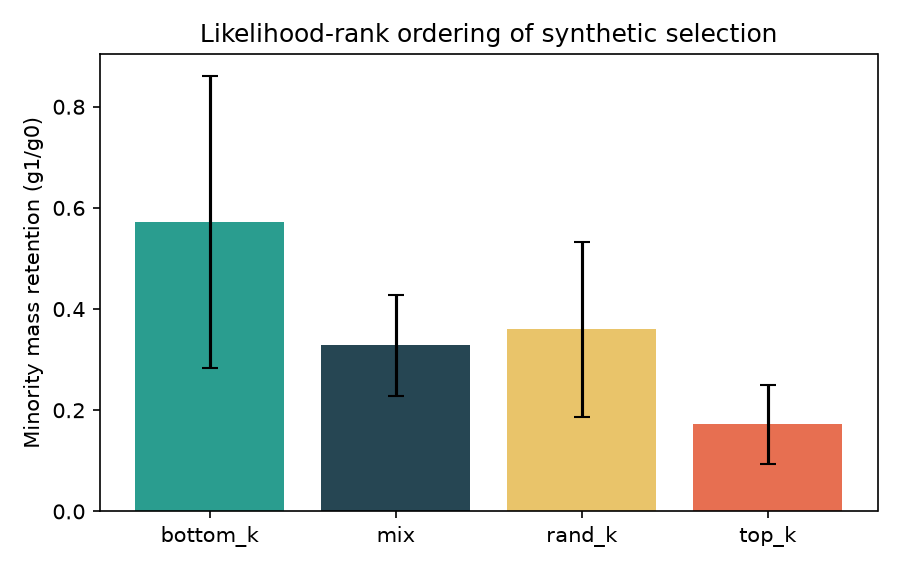
\includegraphics[width=0.48\textwidth]{figures/retention_bars.png}
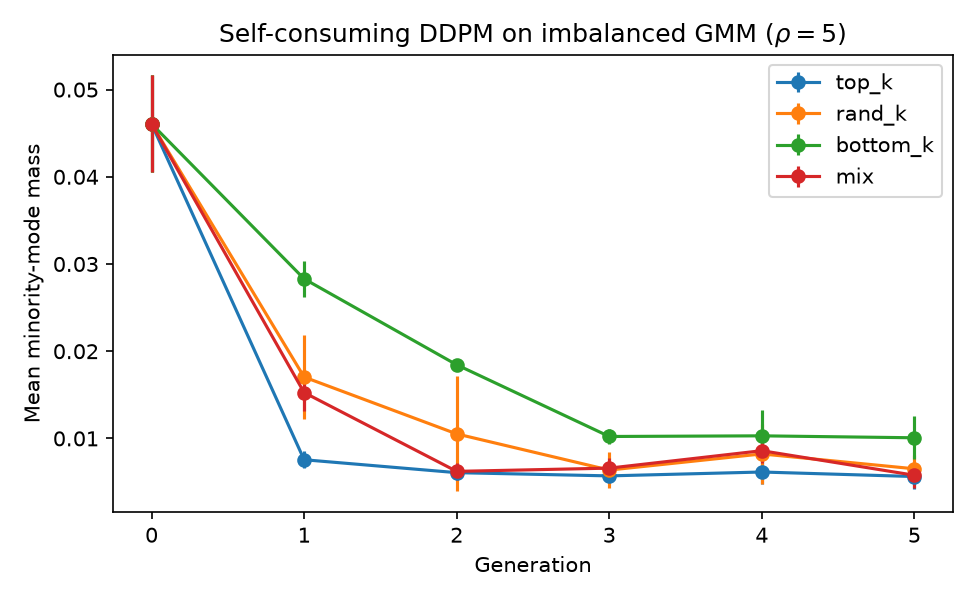
\includegraphics[width=0.48\textwidth]{figures/minority_vs_generation_rho5.png}
\caption{Left: retention by policy on the primary matrix. Right: minority mass vs.\ generation at $\rho{=}5$.}
\label{fig:main}
\end{figure}

\subsection{Sliced $W_2$ (``false stability'' check)}
If top-$k$ were ``falsely stable,'' we would expect better (lower) sliced $W_2$ than random-$k$ while minorities die.
Instead, at generation~1, $\Delta W_2(\mathrm{top}-\mathrm{rand})$ has mean $+0.113$ (std $0.099$), positive on \textbf{all eight} cells (Wilcoxon $p{\approx}0.014$).
Means remain positive for generations $2$--$5$ ($6$--$7$ of $8$ cells; see \texttt{table\_w2\_top\_minus\_rand.csv}).
We report this as \textbf{evidence against} a top-$k$ $W_2$ improvement under minority loss---not as a formal Neyman--Pearson ``falsification'' of a fully specified alternative.

\subsection{Real-mix sensitivity ($\alpha$)}
Separate ablation (\texttt{w2\_fs\_alpha.jsonl}; seeds $\{0,1\}$, $\rho{=}5$, $G{\le}3$):

\begin{table}[t]
\centering
\caption{Mean retention $r$ by real-mix $\alpha$ (two seeds). Order $=$ bottom$>$rand$>$top on both seeds.}
\label{tab:alpha}
\begin{tabular}{lrrrr}
\toprule
$\alpha$ & bottom & rand & top & Order holds \\
\midrule
0.25 & 0.25 & 0.17 & 0.05 & 1/2 \\
0.50 & 0.62 & 0.49 & 0.24 & 2/2 \\
0.75 & 1.34 & 0.77 & 0.94 & 0/2 \\
\bottomrule
\end{tabular}
\end{table}

At $\alpha{\le}0.5$, top-$k$ remains worst; at $\alpha{=}0.75$ the top vs.\ random gap reverses on average while bottom stays highest---an important scope condition ($r>1$ again means minority mass rose vs.\ $g{=}0$).

\subsection{Transfer checks (directional; $n{=}3$)}
These are \textbf{not} powered significance tests; we report mean$\pm$std and seed-wise order counts.
\begin{itemize}
\item \textbf{$8$D GMM} (\texttt{w2\_fs\_hd}): retention $0.55{\pm}0.20$ / $0.27{\pm}0.06$ / $0.08{\pm}0.03$ (bottom/rand/top); order holds $3/3$.
\item \textbf{Digits-PCA} (\texttt{w2\_fs\_digits\_pca}): $1.49{\pm}0.11$ / $1.11{\pm}0.08$ / $0.68{\pm}0.17$; order holds $3/3$.
  Ratios $>1$ mean minority mass increased from $g{=}0$ to $g{=}1$ under bottom/random (definition of $r$ above).
\end{itemize}
An earlier Digits CVAE+classifier probe is inconclusive and unused for claims.

\subsection{Selection-pool size ($k_{\mathrm{frac}}$)}
Under $k=\max(n_{\mathrm{syn}},\lfloor k_{\mathrm{frac}}N\rfloor)$, $k_{\mathrm{frac}}\in\{0.25,0.5\}$ are operationally equivalent when $n_{\mathrm{syn}}$ binds; at $0.75$ top-$k$ remains worst.

\section{Analysis}
Likelihood top-$k$ preferentially retains points the model already explains well (majority modes), reducing minority inflow.
Bottom-$k$ does the opposite relative to random.
Aggregate sliced $W_2$ is a poor monitor for minority survival: it moves with top-$k$ in the wrong direction for a ``quality win.''

\section{Limitations}
\begin{itemize}
\item Toy 2D/8D GMMs and Digits-PCA with tiny networks; not ImageNet-scale.
\item Primary Wilcoxon tests use only $n{=}8$ pairs; uncorrected $p{\approx}0.042$ becomes Holm-adjusted $p{\approx}0.085$. Inference relies on large $d_z$, CIs, and directional consistency.
\item Transfer checks use three seeds without formal hypothesis tests.
\item Digits CVAE transfer was inconclusive; Digits-PCA uses embeddings, not raw pixels.
\item Effect strongest at moderate imbalance and early generations; high real mix ($\alpha{=}0.75$) weakens top vs.\ random.
\item Contribution is a controlled empirical contrast relative to MAD/LSF/Feng, not a new SOTA training method.
\end{itemize}

\section{Conclusion}
Unlabeled likelihood ranking of synthetic data in self-consuming diffusion induces a reproducible minority-retention \emph{order} (bottom-$k$ $>$ random-$k$ $>$ top-$k$) under matched budgets on imbalanced mixtures, with large paired effect sizes despite small $n$.
Top-$k$ does not improve sliced $W_2$ relative to random-$k$ in our primary matrix.
Preferring ``most likely'' synthetics is not a free lunch for minority survival.

\bibliographystyle{plainnat}
\bibliography{refs}

\appendix
\section{Reproducibility and code}
Cross-platform entry point: \texttt{python scripts/reproduce\_w2.py} (also \texttt{scripts/reproduce\_w2.sh} and Windows \texttt{scripts/reproduce\_w2.ps1}).
All numerical tables are produced from logged JSONL via analysis scripts (no hand-edited metrics).
Experiment IDs: \texttt{w2\_fs}, \texttt{w2\_fs\_hd}, \texttt{w2\_fs\_digits\_pca} (supported); \texttt{w2\_fs\_digits} (CVAE; inconclusive).
Source, configs, seeds, and logs are included in the project archive accompanying this manuscript (commit hash recorded in \texttt{SUBMIT.md}); a public GitHub/Zenodo URL will be linked upon posting.

\end{document}
